\chapter{Approach}

\label{Chapter3}

\lhead{Chapter 3. \emph{Approach}}

\section{System overview} % (fold)
\label{sec:system_overview}

The proposed system is constructed around the data flowing through it.

The system takes the data stepwise through an ingestion pipeline, importing, filtering and cleaning it, before churning it into user models. This particular part of the system is elaborated on further in section~\ref{sec:data_ingestion_and_preprocessing}.

Once user models are in place, the system generates user segments. These are stored in a database for future use. There are several viable approaches to the segmentation task. These are discussed in more detail in section~\ref{sec:user_modeling_and_clustering}.

As it turns out, when designing completely autonomous adaptative systems, we need more data than user segments to effectively drive the adaptive component. When considering whether to enable a feature or an interface switch, we need to know whether doing so will be advantageous to the user segment in question. This is discussed in section~\ref{sec:adaptation_component}.

% section system_overview (end)

\section{Data ingestion and preprocessing} % (fold)
\label{sec:data_ingestion_and_preprocessing}

Before the interesting parts of the system can start doing their work, the data needs to be transformed from \emph{a series of chronological raw events} to \emph{a set of user models}.

The amount of data can be arbitrarily sizable, and will grow linearly with user activity. The system architecture has been designed to be able to cope with this; its functional and data-driven nature should be easily adaptable to hugely scalable programming paradigms like MapReduce.

\begin{figure}[h]
  \centering
    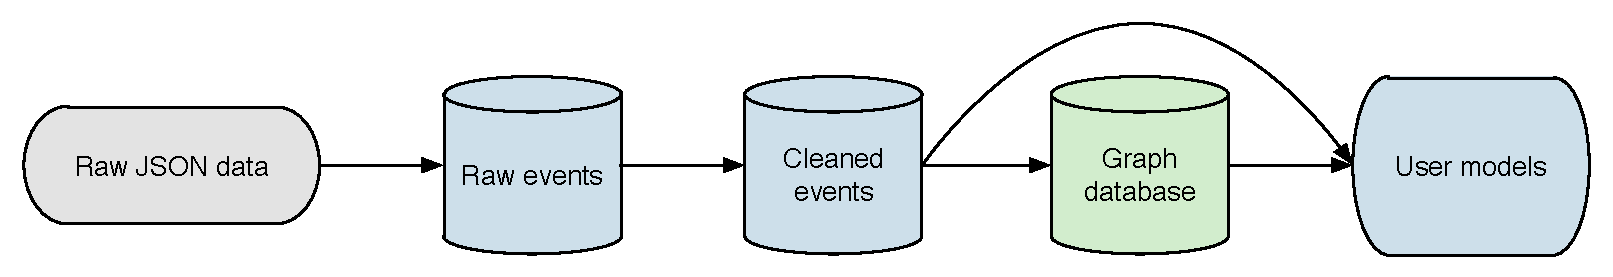
\includegraphics[width=\textwidth]{Figures/ingestion-pipeline}
  \caption{The ingestion pipeline broken into 4 steps. The color of each node indicates means of storage: \emph{Blue} indicates a RDBMS, \emph{green} indicates a graph database, whereas \emph{gray} is used to indicate flat file storage.}
  \label{fig:ingestion-pipeline}
\end{figure}

\subsection{Generating the raw data}
\label{sub:generating_data}

The system input is a chronological series of raw events sent from the production system.

These are instrumented via an external analysis service called KISSmetrics\footnote{\url{https://www.kissmetrics.com/}}. It is a user analysis system designed around tracking individual users' behavior. It works by calling their REST API with the following data:

\begin{enumerate}
  \item person identifier
  \item event name
  \item user properties
\end{enumerate}

The consistency of the personal identifier has already been discussed extensively in the introductory chapters, especially section~\ref{sub:anonymity_privacy}, but a short technical introduction to the actual production system is in order.

\subsection{Event instrumentation in KISSmetrics}
\label{sub:event_instrumentation}

To enable effective utilization of the KISSmetrics instrumentation functionality, they supply a client library for the purpose. This client library handles a few central things for us:

\begin{enumerate}
  \item Person identity storage and loading over subsequent page loads.
  \item The low-level instrumentation of events.
  \item Simple A/B testing facilities.
\end{enumerate}

When the KISSmetrics client library is loaded, the person identity is automatically either retrieved from the browser cookies, or generated.

The identity of a person is a unique randomly generated string, which serves no other purpose than to track the identity of the browser over time. No personal data is stored, nor is it available to us.

Whenever something ``interesting'' happens, an event is sent to the KISSmetrics instrumentation service. An ``interesting'' event is anything that tells us about how the users use the service, both in terms of general activity and in terms of feature adoption. Every event is tagged with the person identity, as well as an event name and a timestamp.

The KISSmetrics service provides several analytical tools to dig into this data, thereamongst funnel reports and cohort reports -- as depicted in figure~\ref{fig:funnel-report} and figure~\ref{fig:cohort-report}.

\begin{figure}[h]
  \centering
    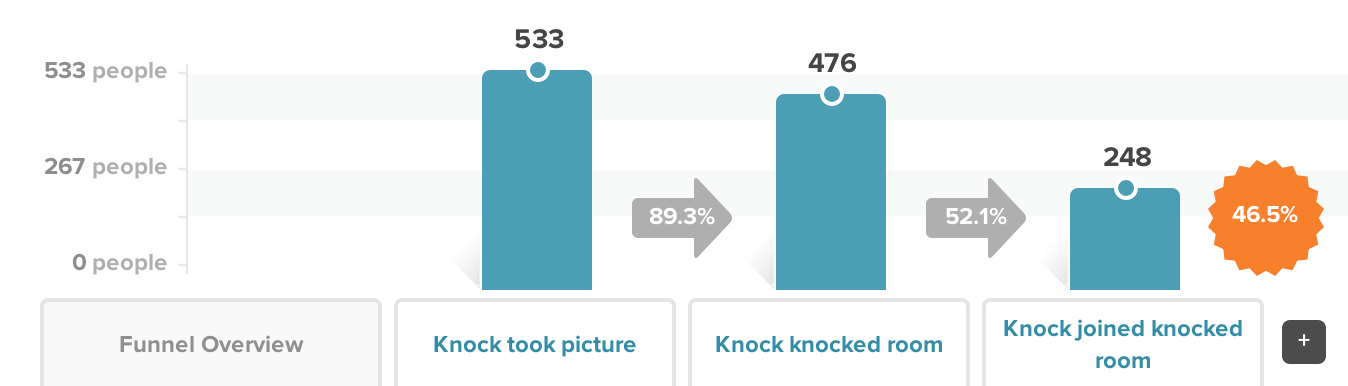
\includegraphics[width=\textwidth]{Figures/screenshots/km/funnel-example}
    \caption{Example of a simple funnel report.}
    \label{fig:funnel-report}
\end{figure}

\begin{figure}[h]
  \centering
    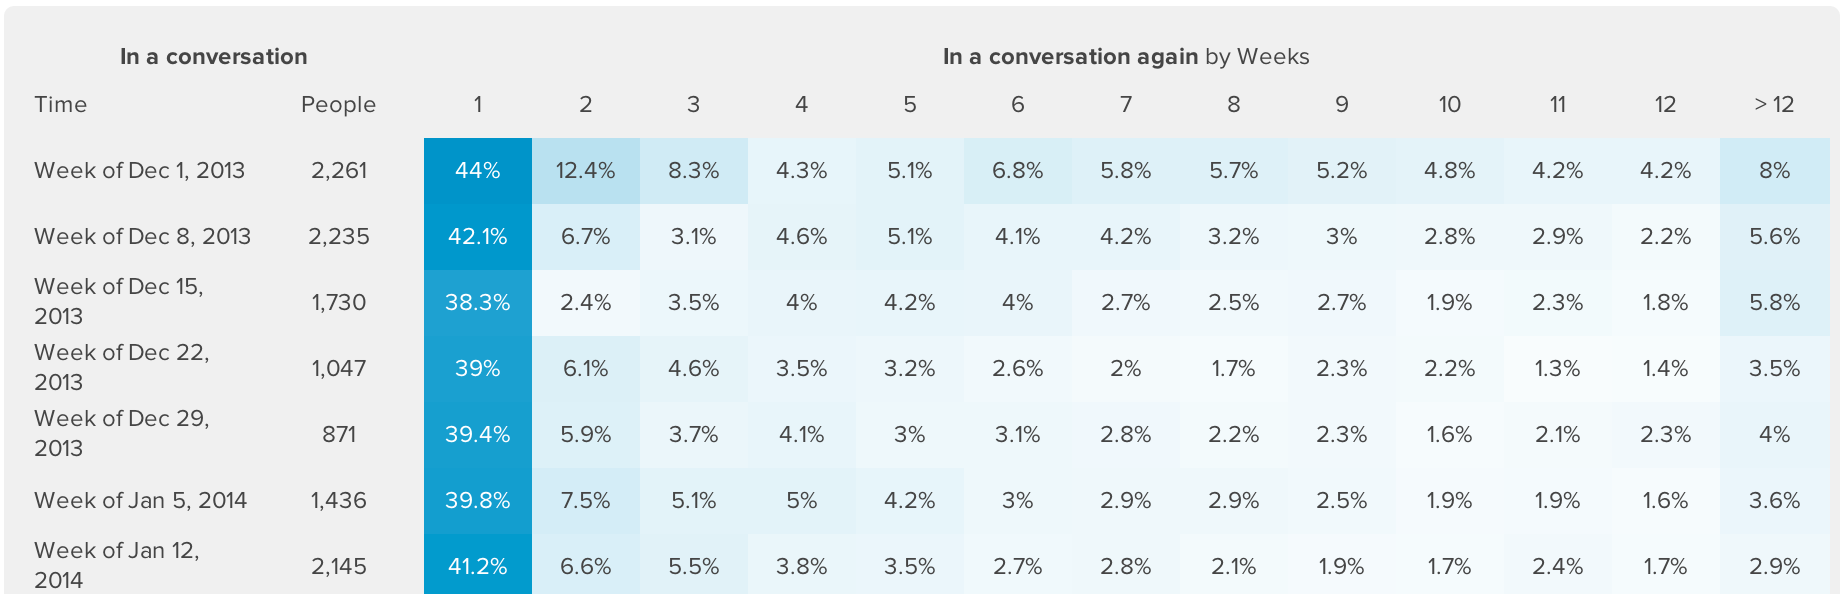
\includegraphics[width=\textwidth]{Figures/screenshots/km/cohort-example}
    \caption{Example of a cohort report.}
    \label{fig:cohort-report}
\end{figure}

% section data_ingestion_and_preprocessing (end)

\section{User modeling and clustering} % (fold)
\label{sec:user_modeling_and_clustering}


Further, whenever

% section user_modeling_and_clustering (end)

\section{Adaptation component} % (fold)
\label{sec:adaptation_component}

\subsection{Evaluation metrics} % (fold)
\label{sub:evaluation_metrics}

\subsubsection{How to measure a positive user experience} % (fold)

% section evaluation_metrics (end)

\subsection{Applying the personalized feature set} % (fold)
\label{sub:applying_the_personalized_feature_set}

Description of the FlagService model.

% section applying_the_personalized_feature_set (end)

\subsection{Tracking user treatments} % (fold)
\label{sub:tracking_user_treatments}

% section tracking_user_treatments (end)

\subsection{Visualizing effects} % (fold)
\label{sub:visualizing_effects}

% section visualizing_effects (end)

% section adaptation_component (end)

\subsection{Differentiating product features} % (fold)
\label{sec:differentiating_product_features}

% section differentiating_product_features (end)

\section{Evolving the user models} % (fold)
\label{sec:evolving_the_user_models}

\subsection{Multi-arm bandits}

\subsection{Tracking individual treatment}

% section evolving_the_user_models (end)

\section{Visualization requirements (?)} % (fold)
\label{sec:visualization_requirements}

% section visualization_requirements (end)
